\subsection{Eigengesichter als Basis}
Im letzten Unterkapitel haben wir den Raum der Differenzgesichter eingeführt.
In diesem Unterkapitel wollen wir eine geeignete Basis dieses Unterraumes finden, nämlich die \textit{Eigengesichter}.
Um uns einige grundlegende Begriffe aus der linearen Algebra in Erinnerung zu rufen, betrachten wir folgende Aufgabe.
\begin{aufgabe}
	Betrachten Sie die Vektoren
	\begin{equation*}
		\vec v_1=\begin{pmatrix}
			\tfrac{3}{5} \\ \tfrac{4}{5} \\ 0
		\end{pmatrix},\quad
		\vec v_2=\begin{pmatrix}
			-\tfrac{4}{5} \\ \tfrac{3}{5} \\  0
		\end{pmatrix},\quad
		\vec v_3=\begin{pmatrix}
			0 \\ 0 \\  1
		\end{pmatrix},\quad
		\vec a=\begin{pmatrix}
			7 \\ 1 \\  4
		\end{pmatrix}.
	\end{equation*}
	\begin{enumerate}[label=(\alph*)]
		\item Die Vektoren $\vec v_1,\vec v_2,\vec v_3$ bilden eine orthonormale Basis von $\mathbb R^3$.
		Begründen Sie warum.
		\item Folglich gibt es genau eine Linearkombination
		\begin{equation*}
			\vec a=c_1\vec v_1+c_2\vec v_2+c_3\vec v_3.
		\end{equation*}
		Berechnen Sie die Koeffizienten $c_1,c_2,c_3$ dieser Linearkombination.
	\end{enumerate}
\end{aufgabe}
\begin{losung*}
	\phantom{text}
	\begin{enumerate}[label=(\alph*)]
		\item Die Vektoren $\vec v_1,\vec v_2,\vec v_3$ sind paarweise orthogonal, also
		\begin{equation*}
			\vec v_1\cdot\vec v_2= \tfrac{3}{5}\cdot\left(-\tfrac{4}{5}\right)+\tfrac{4}{5}\cdot\tfrac{3}{5}+0\cdot 0=0
		\end{equation*}
		und analog findet man $\vec v_1\cdot\vec v_3=0$ und $\vec v_2\cdot\vec v_3=0$.
		Insbesondere sind die Vektoren linear unabhängig.
		Da es drei an der Zahl sind, müssen Sie eine Basis von $\mathbb R^3$ sein.
		Zudem haben die Vektoren Länge Eins, das heisst
		\begin{equation*}
			\vec v_1\cdot\vec v_1= \left(\tfrac{3}{5}\right)^2+\left(\tfrac{4}{5}\right)^2+0^2=1.
		\end{equation*}
		Analog findet man $\vec v_2\cdot\vec v_2=1$ und $\vec v_3\cdot\vec v_3=1$.
		Damit ist diese Basis nicht nur orthogonal, sondern sogar orthonormal.
		\item Da unsere Basis orthonormal ist, kann man die Koeffizienten mit einem Skalarprodukt berechnen.
		Zum Beispiel findet man den Koeffizienten $c_1$ indem man auf beiden Seiten der Gleichung aus der Teilaufgabe das Skalarprodukt mit $v_1$ bildet
		\begin{equation*}
			\vec v_1\cdot\vec a=c_1\underbrace{\vec v_1\cdot\vec v_1}_{=1}+c_2\underbrace{\vec v_1\cdot\vec v_2}_{=0}+c_3\underbrace{\vec v_1\cdot\vec v_3}_{=0},
		\end{equation*}
		also $\vec v_1\cdot\vec a=c_1$.
		Analog erhält man $\vec v_2\cdot\vec a=c_2$ und $\vec v_3\cdot\vec a=c_3$.
		Diese Skalarprodukte berechnen sich zu
		\begin{equation*}
			c_1=5,\quad\quad c_2=-5,\quad\quad c_3=4.
		\end{equation*}
	\end{enumerate}
\end{losung*}

%Die Bilder $\vec a_1,\ldots,\vec a_K$ aus unserer Datenbank sind im Allgemeinen nicht paarweise orthogonal und nicht auf Länge 1 normiert.
Wir werden im Folgenden annehmen, dass die Anzahl der Bilder $K$ viel kleiner ist als die Anzahl der Pixel $M\cdot N$ der einzelnen Bilder.
Der Einfachheit halber nehmen wir zudem an, dass die Vektoren $\vec a_1,\ldots,\vec a_K$ linear unabhängig sind.
Diese bilden dann die Basis eines $K$-dimensionalen Unterraums von $\mathbb R^{M\cdot N}$.
Nun betrachten wir eine weitere Basis dieses Unterraumes, die \textit{Eigengesichter}.
Die Eigengesichter sind eine orthonormale Basis dieses Raumes, wir bezeichnen diese mit $\vec u_1,\dots,\vec u_K\in\mathbb R^{M\cdot N}$.
Diese Basis ist in vielerlei Hinsicht speziell, wie wir sehen werden.
Sie wird aus den Bildern der Datenbank berechnet.
Wenn wir eine andere Datenbank verweden, dann würden die Eigengesichter auch anders aussehen.
Wie diese Berechnung genau geht, werden wir später sehen.
Diese Vektoren können wir wieder als Bilder darstellen.
Das ist in Abbildung~\ref{fig:eigenfaces} gezeigt.

\begin{figure}[ht]
	\centering
	\begin{tabular}{cccccccc}
		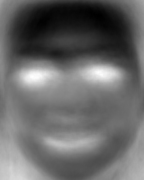
\includegraphics[width=0.1\textwidth]{images/eigenfaces/eigenface00} & 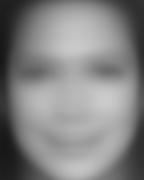
\includegraphics[width=0.1\textwidth]{images/eigenfaces/eigenface01} &
		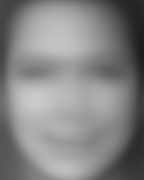
\includegraphics[width=0.1\textwidth]{images/eigenfaces/eigenface02} & 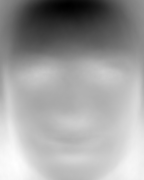
\includegraphics[width=0.1\textwidth]{images/eigenfaces/eigenface03} &
		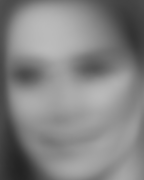
\includegraphics[width=0.1\textwidth]{images/eigenfaces/eigenface04} &
		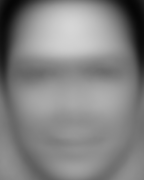
\includegraphics[width=0.1\textwidth]{images/eigenfaces/eigenface05} & 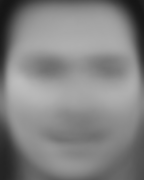
\includegraphics[width=0.1\textwidth]{images/eigenfaces/eigenface06} &
		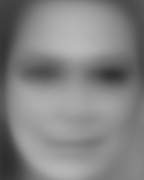
\includegraphics[width=0.1\textwidth]{images/eigenfaces/eigenface07} \\ 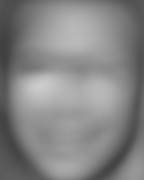
\includegraphics[width=0.1\textwidth]{images/eigenfaces/eigenface08} &
		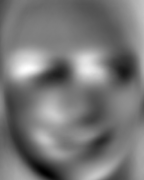
\includegraphics[width=0.1\textwidth]{images/eigenfaces/eigenface09} & 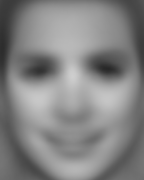
\includegraphics[width=0.1\textwidth]{images/eigenfaces/eigenface10} &
		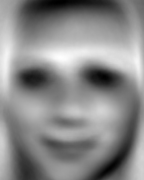
\includegraphics[width=0.1\textwidth]{images/eigenfaces/eigenface11} & 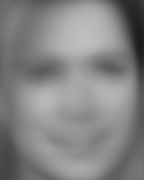
\includegraphics[width=0.1\textwidth]{images/eigenfaces/eigenface12} &
		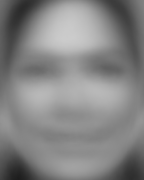
\includegraphics[width=0.1\textwidth]{images/eigenfaces/eigenface13} & 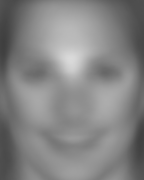
\includegraphics[width=0.1\textwidth]{images/eigenfaces/eigenface14} &
		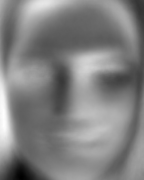
\includegraphics[width=0.1\textwidth]{images/eigenfaces/eigenface15} \\
	\end{tabular}
	\caption{Die ersten 16 Eigengesichter wurden wieder als Bild dargestellt.}
	\label{fig:eigenfaces}
\end{figure}

Wir betrachten nun die Mona Lisa von Leonardo da Vinci, ein Bild das nicht in unserer Datenbank ist.
Auch hier können wir durch Subtraktion von $\vec m$ das Differenzgesicht bilden.
Nun ist es möglich, dieses Differenzgesicht näherungsweise als Linearkombination der Basis $a_1,\ldots,a_K$ oder auch der Basis der Eigengesichter $u_1,\ldots,u_K$ zu schreiben.
Letzteres ist in Abbildung~\ref{fig:eigen_basis} dargestellt.
\begin{figure}[ht]
	\centering
	\begin{tabular}{m{1.8cm} c c c c c m{2cm} c c c m{2cm} c c}
		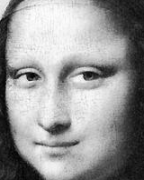
\includegraphics[width=0.1\textwidth]{images/eigenfaces/mona_lisa_original} &
		$-$ & $\vec m$ & $\approx$ & $c_1$ & $\cdot$ & 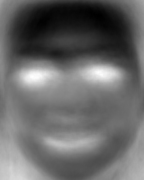
\includegraphics[width=0.1\textwidth]{images/eigenfaces/eigenface00}
		& $+$ & $c_2$ & $\cdot$ & 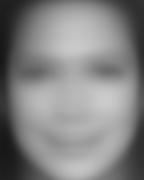
\includegraphics[width=0.1\textwidth]{images/eigenfaces/eigenface01} & $+$ & $\cdots$
	\end{tabular}
	\caption{Differenzgesicht der Mona Lisa als Linearkombination der Eigenfaces.}
	\label{fig:eigen_basis}
\end{figure}
Wir gehen hier nicht näher darauf ein, wie man die Koeffizienten $c_1,\ldots,c_K$ dieser Linearkombination findet (das kommt später).
Wenn mab aber als Basis nicht die Eigengesichter, sondern die Gesichter der Datenbank verwendet hätte, so würden die Koeffizienten anders aussehen, was in Abbildung~\ref{fig:coef} gezeigt ist.
\begin{figure}[ht]
	\centering
	\begin{tabular}{lr}
		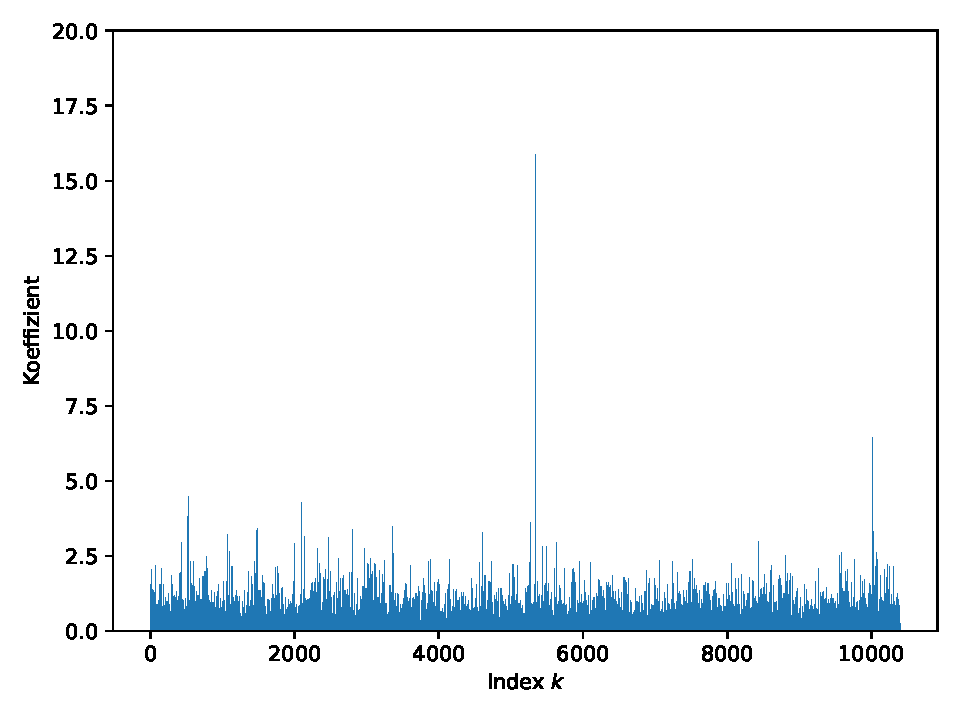
\includegraphics[width=0.45\textwidth]{images/eigenfaces/naive_coef} & 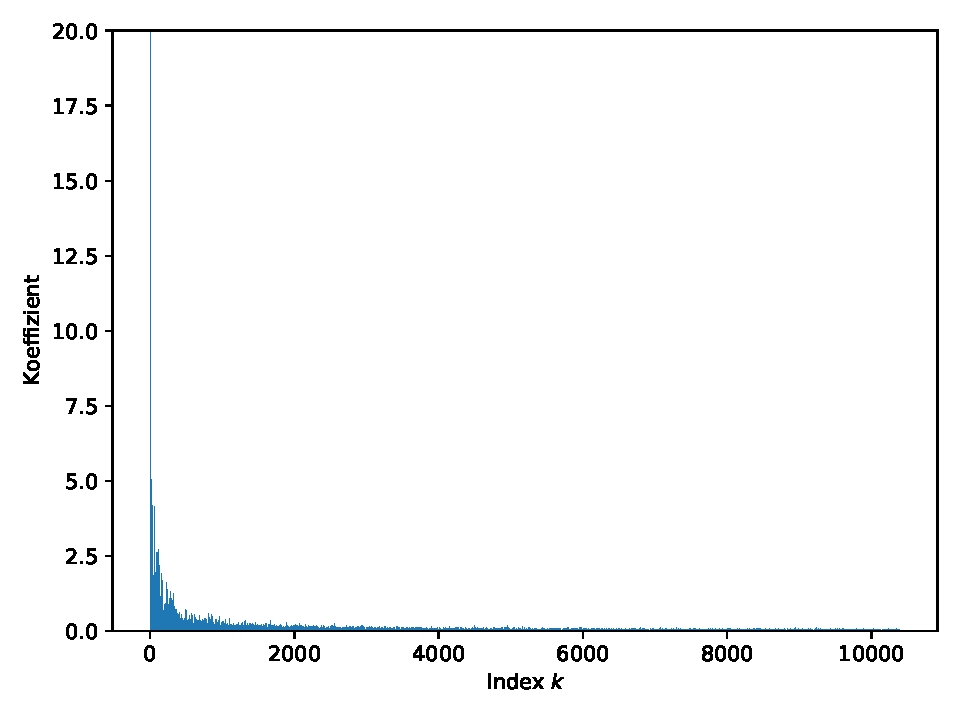
\includegraphics[width=0.45\textwidth]{images/eigenfaces/eigen_coef} \\
	\end{tabular}
	\caption{Der Absolutbetrag der Koeffizienten der Linearkombination des Differenzgesichts der Mona Lisa. Links wurden als Basis die Differenzgesichter der Datenbank und rechts die Eigengesichter genommen.}
	\label{fig:coef}
\end{figure}
\begin{aufgabe}
	Betrachten Sie die Abbildung~\ref{fig:coef}, welche die Koeffizienten der Linearkombinationen bezüglich der beiden Basen zeigt.
	Beschreiben Sie die Unterschiede der Bilder.
	Welche Rückschlüsse kann man dadurch auf die entsprechenden Basen ziehen?
\end{aufgabe}
\begin{losung*}
	Die Koeffizienten der Eigengesichter fallen schnell ab.
	Folglich leisten die ersten $\approx 1000$ Eigengesichter den grössten Beitrag zur Linearkombination.
	Bei der Basis der Differenzgesichter ist keine Solche Struktur zu erkennen.
	In diesem Sinn sind alle diese Differenzgesichter etwa gleich wichtig um das Bild der Mona Lisa darstellen zu können.
\end{losung*}
Was wir hier in Abbildung~\ref{fig:coef} beobachtet haben ist kein Einzelfall.
Obwohl wir nur das Beispiel der Mona Lisa betrachtet haben, würden andere Gesichter ähnlich verteilte Koeffizienten liefern.
Im nächsten Unterkapitel werden wir die Eigengesichter berechnen.
%\begin{figure}[ht]
%	\centering
%	\begin{tabular}{lr}
%		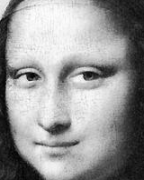
\includegraphics[width=0.2\textwidth]{images/eigenfaces/mona_lisa_original} & 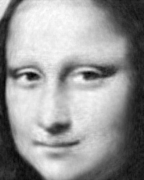
\includegraphics[width=0.2\textwidth]{images/eigenfaces/mona_lisa_2000} \\
%	\end{tabular}
%	\caption{Mona Lisa von Leonardo da Vinci. Links ist das original, rechts ist die Approximation als Linearkombination der ersten 2000 Eigengesichter.}
%	\label{fig:mona_lisa}
%\end{figure}